\documentclass{article}
\usepackage{graphicx}
\usepackage{color}
\usepackage{fullpage}
\usepackage[colorlinks=false]{hyperref}

\begin{document}

\title{Data Visualization and Statistical Graphics in Big Data Analysis}%: What are the modern successors to John W. Tukey's pencil and paper, and mainframe computer, tools?}
\author{Dianne Cook, Department of Statistics, Iowa State Universityy\\
Eun-Kyung Lee, EWHA\\
Mahbubul Majumder, University of Nebraska-Omaha}
\date{These are the thoughts that I have for pulling together the article on Visualization of Big Data for the Annual Reviews. }
\maketitle

In the 1970s J. W. Tukey introduced the world to exploratory data analysis -- data visualization was a major component of this area. Some of his famous quotes point to the reasons for the importance of statistical graphics:

\begin{quote}
{\em Good pictures of data ``force the unexpected upon us.'' } (J. W. Tukey)
\end{quote}

\noindent and he was also an early adopter of harnessing technology for data analysis, and 45 years ago foretold today's technological big data world:

\begin{quote}
{\em ``Today, software and hardware together provide far more powerful factories than most statisticians realize, factories that many of
today's most able young people find exciting and worth learning about on their own''}
\end{quote}

I have heard twice in the last two months from successful data mining teams: the key to their model winning the competition was the data pre-processing involving a lot of data plots that helped them to understand what they were working with, and problems with the data that needed to be addressed before being able to make effective models. This is important for big data, how to effectively clean, transform and pre-process large complex data sets. Visualization plays a key role. This is just as important for big data as it was for John Tukey's days, and the technology has radically changed. 

What I'd like to do for the big data visualization review paper is to focus on the importance of plotting data to learn things that were not expected, and to improve data analysis and modeling. 

\begin{itemize} \itemsep 0in
\item Very short intro to the spirit of EDA, as was practiced by J. W. Tukey.

\item How technology has changed the landscape of EDA

\item Work that has come between Tukey and the young researchers of today, focusing on people who may not have received a lot of attention: Andreas Buja, Antony Unwin, Chris Wild, John Maindonald, Debby Swayne, Hadley Wickham, Yihui Xie. 

\item What are the building blocks for his successors today: R and bioconductor, enable everyone to participate; reshaping data, data wrangling, split-apply-combine, 

\item The largest chunk will be examples from people who have won major big data analysis competitions in the past year, how visualization played a role,  what plots they made and what they learned from them, that helped to improve the model results. 

\item Interplay between exploratory and inferential statistics, how to couple discovery of structure with assessment of how real the patterns are. 

\item Also will review relevant publications in major journals: TAS, JCGS, Computational Statistics, Statistical Science, JASA, JSS, ... that show new graphics methodology.

\end{itemize}

John Tukey's EDA, and the tools for plotting your data are all around us today, but knowledge of how to effectively leverage visualization is not widespread or effectively incorporated into statistics curricula. 

\section{Data Competition Success Due to Data Visualization}

\subsection{Kaggle Health Heritage Prize}

In April, 2011 Kaggle posted the details of the Heritage Health Prize ``Improve Healthcare, Win \$3,000,000".  Dr Phil Brierley was part of the three person team that won the first two milestone awards of \$230,000, and combined forces with another team to win the final prize of \$500,000. This competition is an example of big data challenges of today: large amounts of data on hospital admissions being used to develop models to improve the efficiency of healthcare spending. In interviews post-prize, he echoes of Tukey's long ago words:

\begin{quote}
{\em ``In many of the analytics problems I have been involved in, the problem you end up dealing with is not the one you initially were briefed to solve.
These new problems are always discovered by visualising the data in some way and spotting curious patterns." }\url{http://www.anotherdataminingblog.blogspot.co.uk/2011/12/whats-going-on-here.html} 
\end{quote}

Here is an example from Dr Brierley's blog, that illustrates a algorithmic trading challenge. Figure \ref{liqshock} shows a plot made of timing of ``liquidity shocks'' in data from the London Stock Exchange. There is something going on a 2:30pm, 3:30pm and 4pm. This can only be seen when all commodities are looked at together. Perhaps it is people going to lunch, coffee breaks, timing of the opening of other stock exchanges. Using time alone is dangerous because it is most likely event-related, which may change to other times with new data. Without determining the causes of these spikes modeling them is not robust, and it looks like for this reason Dr Brierley decided that this competition was not worth entering because the data was inadequate. 

\begin{figure*}
\centerline{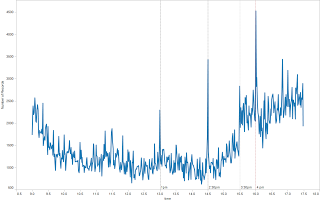
\includegraphics[width=4in]{images/shockeventtimings.png}}
\caption{Times of ``liquidity shocks" in data from the London Stock Exchange. (Reprinted with permission from \url{http://www.anotherdataminingblog.blogspot.co.uk/2011/12/whats-going-on-here.html})}
\label{liqshock}
\end{figure*}

\subsection{Data Mining Cup}

Each year Prudsys AG  challenges students with  the Data Mining Cup competition. In 2014, the problem was announced to student team on April 2, and students needed to have their final entry by May 14. The student teams had six weeks to develop a solution for a data mining problem on the topic of optimal return prognosis. More specifically, the goal was to use an online shop�s historical purchase data to come up with a model for new orders that would calculate the probability of a purchase leading to a return. In this year's competition, a team of students (Guillermo Basulto-Elias (statistics), Fan Cao (statistics), Xiaoyue Cheng (statistics), Marius Dragomiroiu (computer science), Jessica Hicks (bioinformatics and computational biology), Cory Lanker (statistics), Ian Mouzon (statistics), Lanfeng Pan (statistics) and Xin Yin (bioinformatics and computational biology/statistics) from Iowa State University was the first north American team to win. A key component of that win was the pre-processing of the data, that utilized substantial graphics to learn about their data, and inform their modeling. 

Figure \ref{DMC1} shows one plot used early by the ISU DMC team, to examine return rates by time and product. Yellow indicates most of the ordered items where kept, blue means they were mostly returned and pink are items to be predicted. Two major structures are immediately visible, new product introductions in July 2012 and January 2013. The other major structure is that new data to be predicted was in the third season of the time period, and this information was crucial to construct good training and test sets for model building. 

\begin{figure*}
\centerline{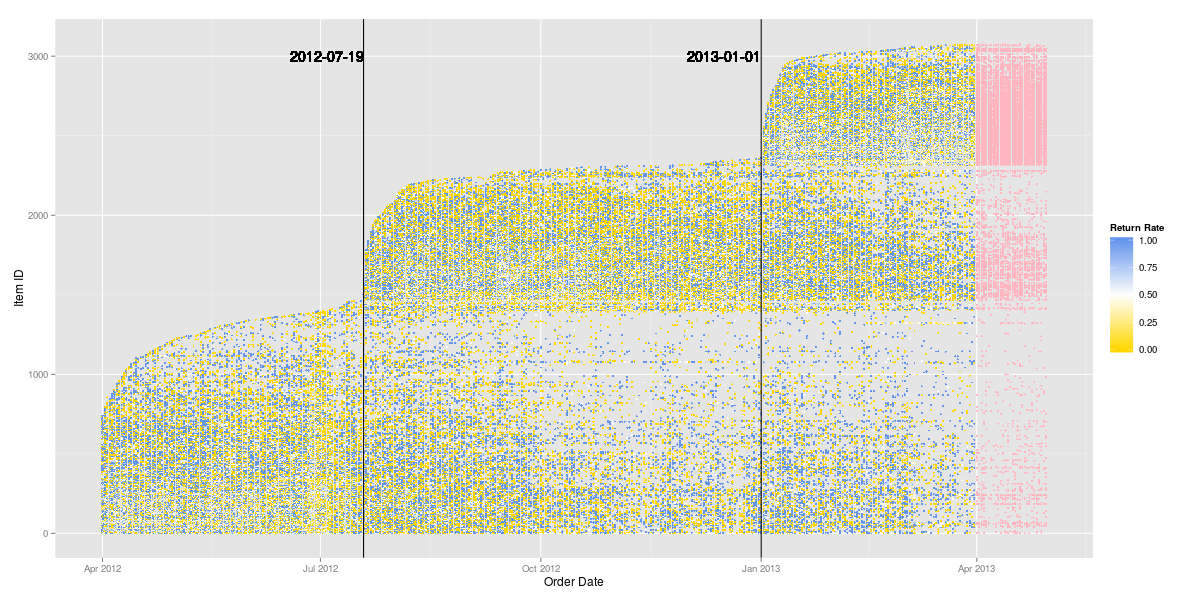
\includegraphics[width=7in]{images/orderDate_itemID.png}}
\caption{One of the preliminary plots made by the ISU DMC team. Item ID plotted against order date, colored by return rate. }
\label{DMC1}
\end{figure*}

\end{document}

% John Deere, Andy Roberts

% Data Mining Cup team

% Phil Brierley


